\documentclass[a4paper,11pt,final]{article}
\usepackage{hyperref}
\usepackage{graphicx}
\usepackage{minted}

\begin{document}

\title{Pweave Example - Frequency response of a moving average filter}
\author{Matti Pastell \\
\url{http://mpastell.com}}

\maketitle

\textbf{Create 11 point moving average filter and plot its frequency response and print the values.}


\begin{minted}[mathescape, fontsize=\small, xleftmargin=0.5em]{python}
from pylab import *
import scipy.signal as signal
#A function to plot frequency and phase response
def mfreqz(b,a=1):
    w,h = signal.freqz(b,a)
    h = abs(h)
    return(w/max(w), h)\end{minted}


\textbf{Make the impulse response function and use terminal formatted output (=doctest block.)}


\begin{minted}[fontsize=\footnotesize, xleftmargin=0.5em, mathescape]{python}
>>> n = 11.
>>> n
11.0
>>> b = repeat(1/n, n)
>>> b
array([ 0.09090909,  0.09090909,  0.09090909,  0.09090909,  0.09090909,
        0.09090909,  0.09090909,  0.09090909,  0.09090909,  0.09090909,
        0.09090909])
\end{minted}



\textbf{Calculate the frequency response and plot it:}


\begin{minted}[mathescape, fontsize=\small, xleftmargin=0.5em]{python}
w, h = mfreqz(b)
#Plot the function
plot(w,h,'k')
ylabel('Amplitude')
xlabel(r'Normalized Frequency (x$\pi$rad/sample)')
show()\end{minted}
\begin{figure}[htpb]
\center
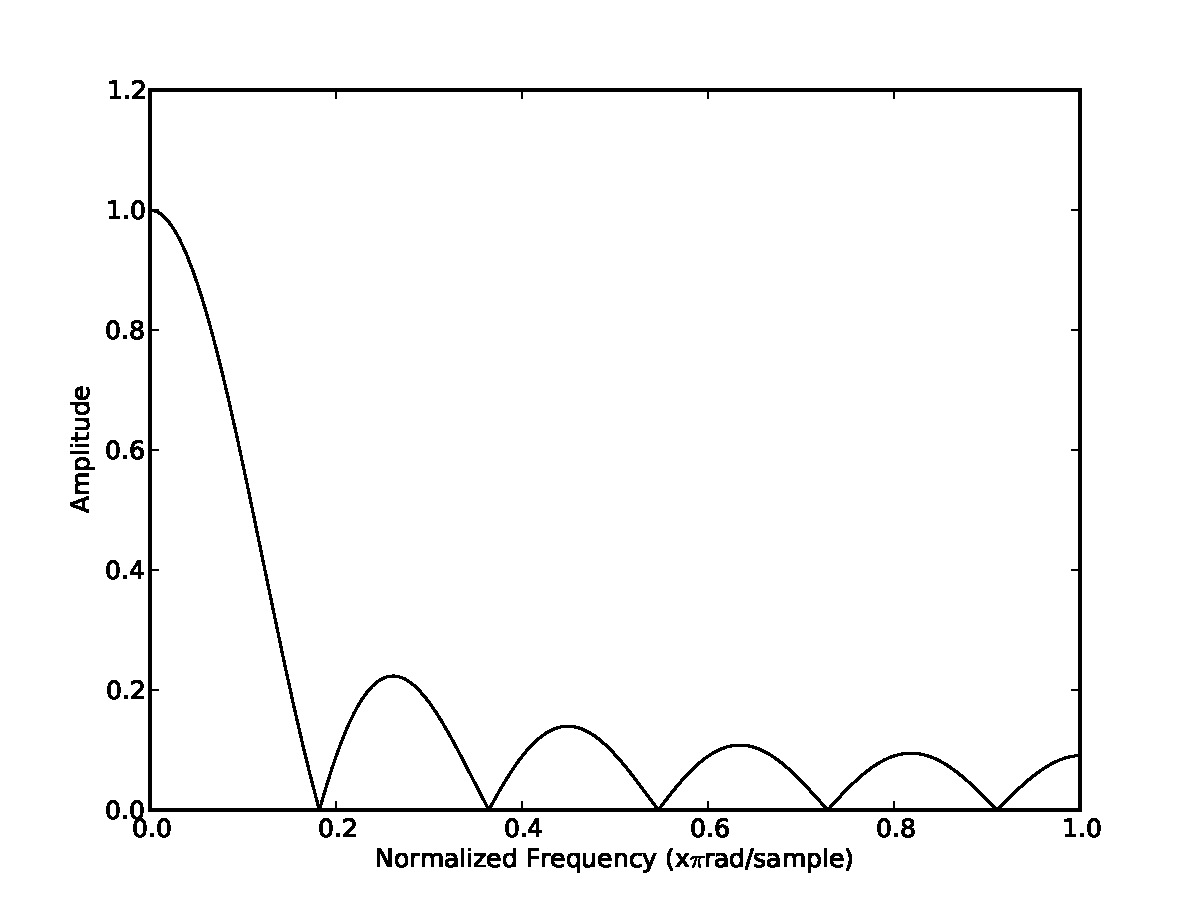
\includegraphics[width= \textwidth]{figures/ma-tex_figure3_1.pdf}
\caption{Frequency response of an 11 point moving average filter}
\label{fig:None}
\end{figure}




\begin{table}
\caption{The first 10 values of the frequency response (w,h) as a table, notice that the code is hidden in the output document.}
\begin{center}
\begin{tabular}{ c | c }
\hline
\textbf{Amplitude} &  \textbf{Frequency} \\ \hline



1.0 & 0.0 \\
1.0 & 0.0 \\
1.0 & 0.0 \\
1.0 & 0.01 \\
1.0 & 0.01 \\
1.0 & 0.01 \\
0.99 & 0.01 \\
0.99 & 0.01 \\
0.99 & 0.02 \\
0.98 & 0.02 \\

\end{tabular}
\end{center}
\end{table}

\end{document}
 
